\maketitle
\newpage


\newcommand{\consultation}[1]{%
    \thispagestyle{empty}
    \ifnum #1 = 0
        This dissertation may be made available for consultation within the
        University Library and may be photocopied or lent to other libraries
        for the purposes of consultation.
    \else
        This dissertation may not be consulted, photocopied or lent to other
        libraries without the permission of the author for #1 
    \ifnum #1 = 1
        year
    \else
        years
    \fi
        from the date of submission of the dissertation.
    \fi
    \vspace{4em}

    Signed:
}
\consultation{0}
\newpage


\newcommand{\declaration}[2]{
    \thispagestyle{empty}
    \begin{center}
        \LARGE\textbf{#1}
    \end{center}
    \begin{center}
        Submitted by: #2
    \end{center}
    \section*{COPYRIGHT}
        Attention is drawn to the fact that copyright of this dissertation rests
        with its author. The Intellectual Property Rights of the products
        produced as part of the project belong to the author unless otherwise specified
        below, in accordance with the University of Bath's policy on intellectual property 
       (see http://www.bath.ac.uk/ordinances/22.pdf).

        This copy of the dissertation has been supplied on condition that anyone
        who consults it is understood to recognise that its copyright rests with its
        author and that no quotation from the dissertation and no information
        derived from it may be published without the prior written consent of
        the author.

    \section*{Declaration}
        This dissertation is submitted to the University of Bath in accordance
        with the requirements of the degree of MComp (hons) Computer Science and Mathematics in the
        Department of Computer Science. No portion of the work in this dissertation
        has been submitted in support of an application for any other degree
        or qualification of this or any other university or institution of learning.
        Except where specifically acknowledged, it is the work of the author.

        Signed:
}
\declaration{Natural Proof Search for Classical Logic}{Adam Lassiter}
\newpage


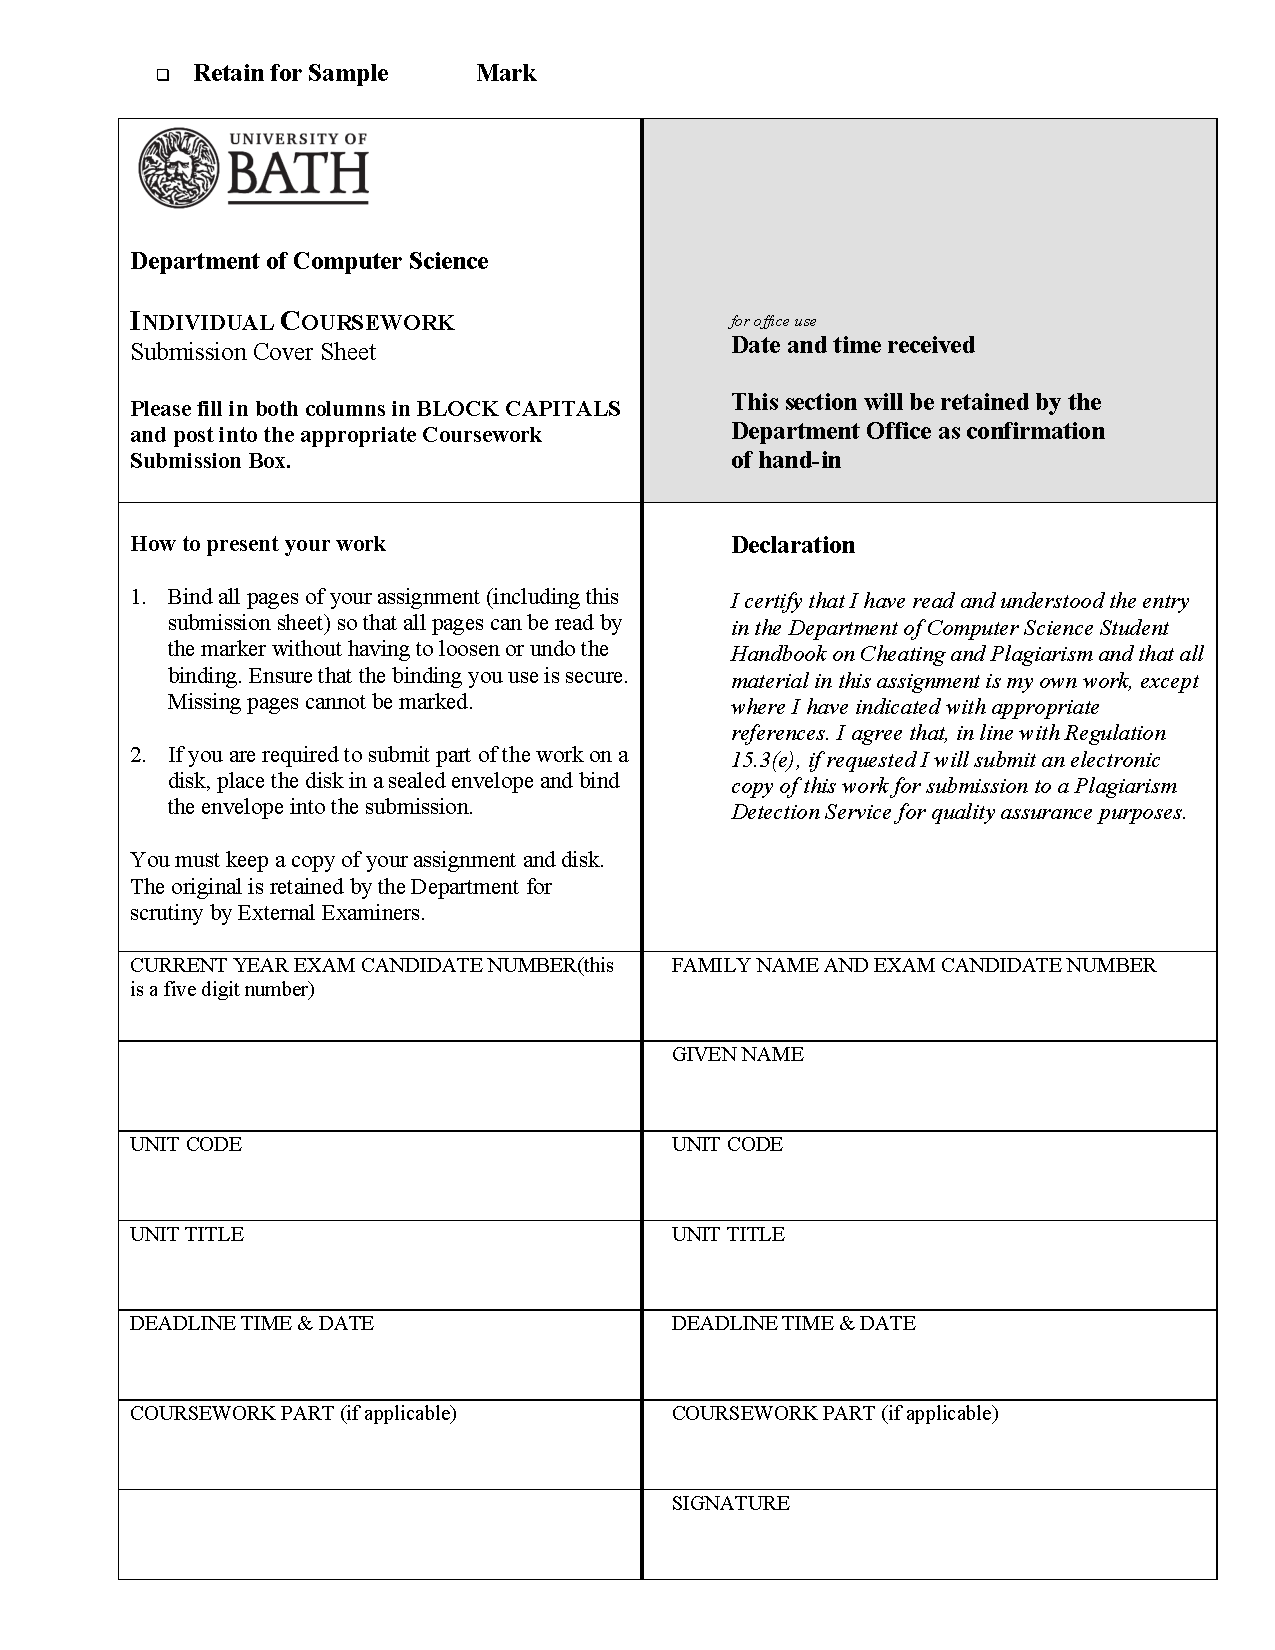
\includepdf{coversheet.pdf}


\abstract
    We investigate a natural algorithm for proof search within classical logic and bounds on the complexity class of such a search.
    We further examine natural optimisations to this algorithm and how they affect complexity bounds.
\newpage

\section*{Acknowledgements}
    Herein is the conclusion to four years of university study and seven months of study on proof search and additive linear logic sequent proofs.
    Written in support of the final year of MComp (hons) Computer Science and Mathematics degree at University of Bath, it has led me through many ups and downs, constantly tackling new problems and potential solutions.
    For all the wonder and difficulties surrounding P versus NP problems, this points another finger the way of `not equal' but further research and proof remains to be seen.
    Fortunately, I feel this provides a remarkable approach to a human-understandable and natural proof search, providing links between previous methods and may help build a deeper understanding.

    I would like to express my gratitude to Dr. Willem Heijltjes for his enthusiasm, guidance and words of wisdom throughout, always bright-eyed at the prospect of new discoveries.
    I further extend my gratitude to all those who kept me motivated throughout, enduring my endless `rubber-duck debugging' and guiding me through the finer points of English grammar.

    Happy reading,\par
    Adam Lassiter
\newpage


\tableofcontents
\newpage

%% \listoffigures
%% \newpage
%% 
%% \listoftables
%% \newpage



